% !TEX program = xelatex

\documentclass[10pt,aspectratio=169]{beamer}
\usetheme[
    hidetitle,           % hide the (short) title in the sidebar
    hideauthor,          % hide the (short) author in the sidebar
    hideinstitute,       % hide the (short) institute in the bottom of the sidebar
    left                 % right of left position of sidebar
  ]{Aalborg}

\setbeamercolor{alerted text}{fg=beamer@headercolor}

\usepackage[ngerman]{babel}
\usepackage[babel,german=guillemets]{csquotes}
\usepackage{datetime}
\usepackage[version=4]{mhchem}
\usepackage{booktabs}
\usepackage{xspace}
\usepackage{multicol}
\usepackage{graphicx}
\usepackage{tikz}
\usepackage{hyperref}
\newcommand{\doi}[1]{\href{https://doi.org/#1}{doi:#1}}


%\setbeamercolor{section in sidebar current subsection}{use=section in sidebar,fg=section in sidebar.fg,bg=section in sidebar.bg}
% Grafikpfad direkt in den figures-Ordner der Dissertation leiten
\graphicspath{{../figures/}}

\usepackage{fontspec}
\usepackage{lmodern}
\IfFileExists{../font/LinotypeSyntaxCom-Regular.ttf}{
  \setsansfont{LinotypeSyntaxCom}[
    Path=../font/,
    Extension = .ttf,
    UprightFont=*-Regular,
    BoldFont=*-Bold,
    ItalicFont=*-Italic,
    BoldItalicFont=*-BoldIt
  ]
}{
  \usepackage{lmodern}
}

\usepackage{animate}
\usepackage[version=4]{mhchem}
\usepackage{orcidlink}

% Dummy-Befehl für eventuelle Hintergrundbilder aus der Vorlage
%\newcommand{\BUWtitlebg}{}

\title[Dissertation]
{Advanced 2D and 3D characterisation of clinker phases and hydrated cementitious binders}

\subtitle{Inhaltsübersicht der Dissertation}
\date{10. Juni 2026}

\newcommand\shortauthor{Florian Kleiner}
\newcommand\orcid{0000-0001-6002-0829}
\author[\shortauthor]{
  \shortauthor\,\orcidlink{\orcid}\\
  \href{mailto:florian.kleiner@uni-weimar.de}{{\tt florian.kleiner@uni-weimar.de}}
}

\institute[Bauhaus-Universität Weimar]{
  Bauhaus-Universität Weimar\\
  Fak. B\&U\\
  Prof. Werkstoffe des Bauens
}

\begin{document}

% ---------------------------------------------------
% Folie 1: Titelfolie
% ---------------------------------------------------
{\BUWtitlebg
\begin{frame}[plain,noframenumbering]
  \titlepage

\end{frame}}


\section{Motivation}
\begin{frame}{Motivation \& Zielsetzung}
  \begin{itemize}
    \item Die Zementhydratation ist ein hochkomplexer Prozess.
    \item Klassische Einzelmethoden stoßen bei der Auflösung von Nano-Porenräumen, Spurenelementen oder der Phasenzuordnung an ihre Grenzen.
  \end{itemize}
  
  \begin{center}
    \animategraphics[palindrome,autoplay,width=.75\textwidth]{6}{intro-anim/Animation}{01}{10}
  \end{center}
\end{frame}

\section{Methoden}
\begin{frame}{Methoden}
  \textbf{Ziel ist die Überwidnung dieser Grenzen durch}
  \begin{itemize}
    \item Einsatz korrelativer Mikroskopie,
    \item Automatisierung von Auswertungen und Bildanalysen,
    \item Vergleich verschiedener Methoden,
  \end{itemize}
  \begin{center}
    \begin{tabular}{lll}
      \toprule
      \textbf{Präparation} & \textbf{Bildgebend} & \textbf{Physikalisch} \\
      \midrule
      ArBIB & REM-BSE/SE & Nanoindentation (NI) \\
      Kryo-FIB & EDX \& EBSD & LT-DSC \\
      fs-Laser & LA-ICP-MS & MIP \\
       & FIB-nT & \\
      \bottomrule
    \end{tabular}
  \end{center}
  \begin{itemize}
    \item Fokus auf den Erhalt der nativen Mikrostruktur.
  \end{itemize}
\end{frame}


\section{Präparation mit ArBIB}
\begin{frame}{Argon Broad Ion Beam (ArBIB) Böschungsätzen}
  \begin{columns}
    \begin{column}{0.5\textwidth}
      \begin{itemize}
        \item Großflächige Politur hydratisierter Proben ohne Einbetten.
        \item Mit Einbettung verbesserte Porensegmentierbarkeit.
        \item Ermöglicht Visualisierung von Nanoporen im dichten C-S-H Gefüge.
        \item Kryo-ArBIB reduziert Temperaturschäden an Hydratphasen.
      \end{itemize}
    \end{column}
    \begin{column}{0.5\textwidth}
      \centering
      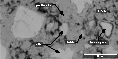
\includegraphics[width=\linewidth]{literature/ArBIB-CEMI-BSE.pdf}\\
      \footnotesize ArBIB-polierter, 28\,d hydratisierter CEM I\\ % fig:LAICPMS-positions

    \end{column}
  \end{columns}
   \vfill\raggedleft\tiny\itshape F. Kleiner, C. Matthes, C. Rößler,`Argon broad ion beam sectioning and high resolution scanning electron microscopy imaging of hydrated alite', 2021, \doi{10.1016/j.cemconres.2021.106583}%kleiner.2021a
\end{frame}


\section{Korrelative Mikroskopie}
\subsection{BSE + EDX + LA-ICP-MS}
\begin{frame}{Spurenelementanalyse im Klinker}
  \begin{columns}
    \begin{column}{0.5\textwidth}
      \textbf{BSE + EDX + LA-ICP-MS}
      \begin{itemize}
        \item Gute Auflösung der EDX-Daten ermöglicht exakte Phasen-Zuordnung der LA-ICP-MS-Messungen.
        \item Spurenelemente wie V, Ba, Rb konzentrieren sich im \ce{C2S}, Ti und Mn in den Zwischenphasen.
      \end{itemize}
    \end{column}
    \begin{column}{0.5\textwidth}
      \centering
      \animategraphics[loop,autoplay,width=\linewidth]{1}{la-icp-ms/position2-anim/Animation}{0}{4}\\
      \footnotesize Position der EDX- und LA-ICP-MS-Messungen.\\ % fig:LAICPMS-positions

    \end{column}
  \end{columns}
   \vfill\raggedleft\tiny\itshape F. Kleiner, M. Decker, C. Rößler, H. Hilbig, H.-M. Ludwig,`Combined LA-ICP-MS and SEM-EDX analyses for spatially resolved major, minor and trace element detection in cement clinker phases', 2022, \doi{10.1016/j.cemconres.2022.106875}% kleiner.2022b
\end{frame}

\subsection{Nanoindentation + EDX}
\begin{frame}{Nanoindentation (NI) + EDX}
  \begin{columns}
    \begin{column}{0.5\textwidth}
      \textbf{Mechanische Eigenschaften von Mörteln}
      \begin{itemize}
        \item Präparation mittels ArBIB
        \item geringere Präparationsartefakte (Vermeidung von Reliefs)
        \item Kombination von NI + EDX
        \item Direkte, detaillierte Phasenzuordnung von Härte/Modul (z.\,B. Quarz, \ce{C3S}, \ce{C2S}, C-S-H, C-A-S-H) im Gegensatz zum sonst groben Dekonvolutionsverfahren
      \end{itemize}
    \end{column}
    \begin{column}{0.5\textwidth}
      \centering
      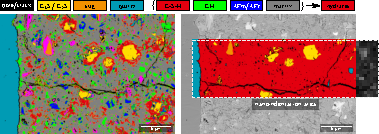
\includegraphics[width=.8\linewidth]{nanoindentation/EDX_positions.pdf}\\
      \footnotesize EDX Phasenkarte, registriert auf einem BSE-Bild\\am Ort der NI-Versuche.\\
      \vspace{0.15cm}
      %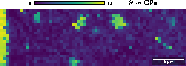
\includegraphics[width=.8\linewidth]{nanoindentation/NI2D_results_H.pdf}\\
      \animategraphics[loop,autoplay,width=.8\linewidth]{1}{./graphics/NI/0}{0}{2}\\
      \footnotesize EDX Phasenkarte, registriert auf Härte-Map ($H$)\\% fig:ni2D-results
    \end{column}
  \end{columns}
  \vfill\raggedleft\tiny\itshape unpublished
\end{frame}



\section{Hydratsaum- und Abstandsmessung}
\subsection{Hydratsaummessung}
\begin{frame}{Automatisierte Hydratsaummessung (HLT)}
  \begin{columns}
    \begin{column}{0.5\textwidth}
      \begin{itemize}
        \item Entwicklung eines Algorithmus zur HLT-Messung an großen BSE Bildern.
        \item Über Koordinatentransformation (kartesisch zu polar).
        \item Ermöglicht die Messung des Hydratationsfortschritts an Hunderttausenden von Partikeln.
      \end{itemize}
    \end{column}
    \begin{column}{0.5\textwidth}
      \centering
      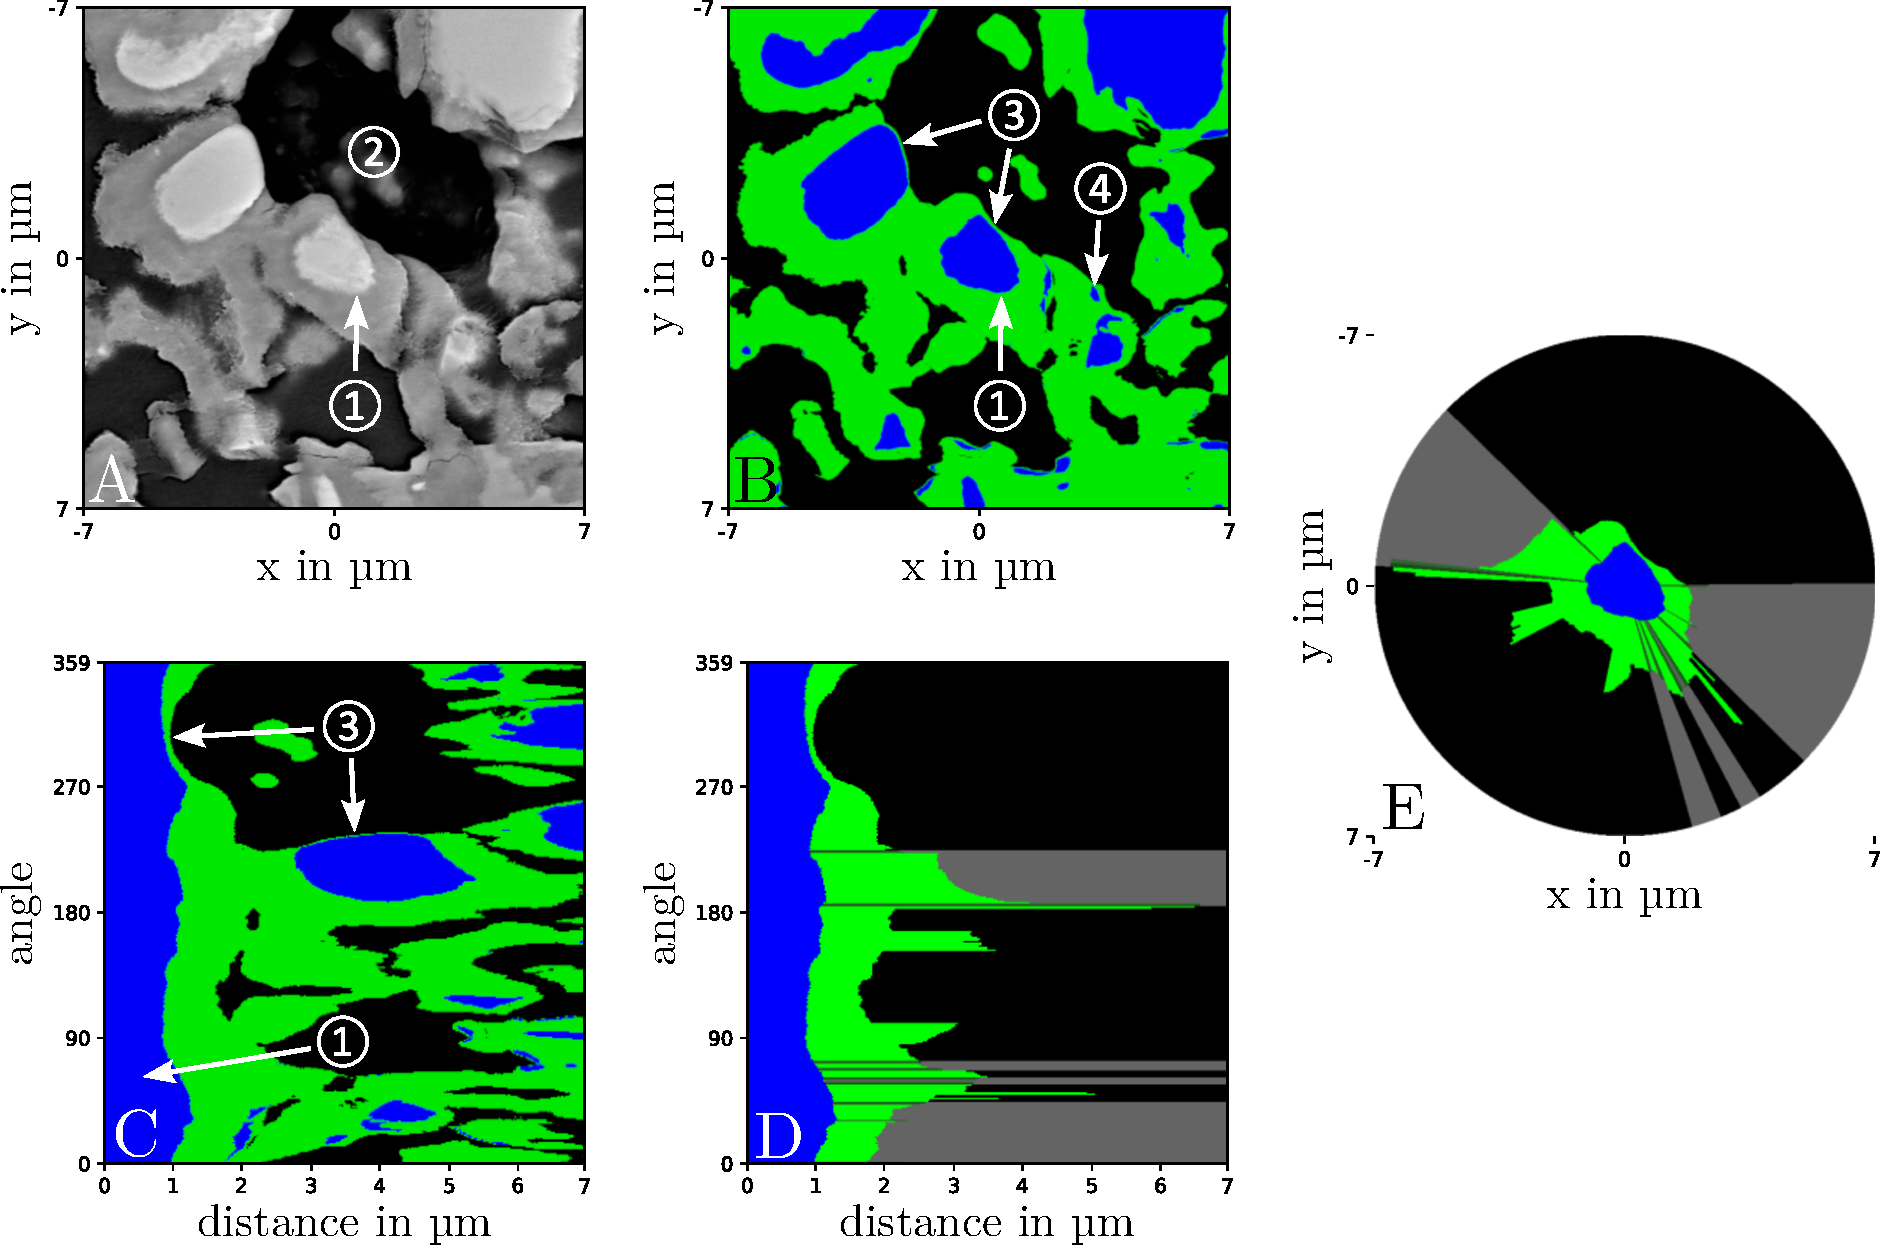
\includegraphics[width=0.9\linewidth]{hydrate-rim/Mechanism_v2.pdf} % fig:hlt-method
      \footnotesize Illustration der HLT-Messung\\am Beispiel eines Klinkerkorns.
    \end{column}
  \end{columns}
   \vfill
   \raggedleft\tiny\itshape F. Kleiner, F. Becker, C. Rößler, H.-M. Ludwig,`A Python tool to determine the thickness of the hydrate layer around clinker grains using SEM-BSE images.', 2024, \doi{10.1111/jmi.13283}%kleiner.2024a
\end{frame}


\begin{frame}{Automatisierte Hydratsaummessung (HLT)}
  \begin{columns}
    \begin{column}{0.5\textwidth}
      \textbf{Ergebnis für \ce{C3S} und \ce{C2S}:}
      \begin{itemize}
        %\item Bis zu 28\,d alte Proben lassen eine Messung zu.
        \item Für Reinphasen (\ce{C3S} und \ce{C2S}) ist das HLT-Wachstum bis zu 28 Tage alten Proben messbar.
        \item \ce{C2S} zeigt erwartbar langsameres C-S-H-Wachstum als \ce{C3S}.
        \item Für Mischphasen (\ce{C3S}:\ce{C2S} 3:1, 1:1, 1:3) lassen sich unterschiedliche Wachstumsraten um \ce{C3S} und \ce{C2S} feststellen.
      \end{itemize}
    \end{column}
    \begin{column}{0.5\textwidth}
      \centering
      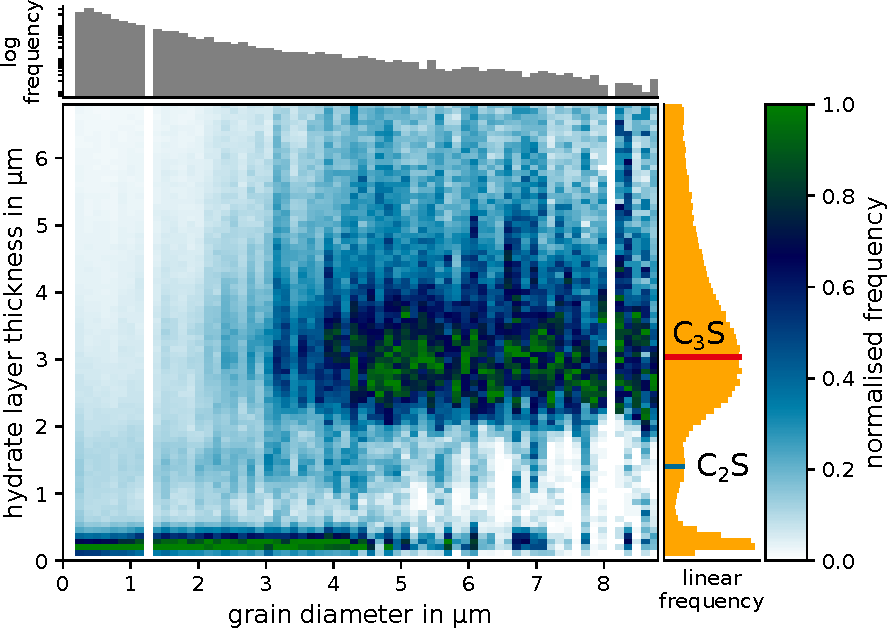
\includegraphics[width=\linewidth]{hydrate-rim/HLT_histogram_3-1.pdf} % fig:hlt_mixture_peaks
      \footnotesize HLT-Ergebnis für 28\,d hydratisiertes \ce{C3S}:\ce{C2S} 3:1. Im HLT-Histogramm (orange) lassen sich\\die Peaks (grün) \ce{C2S} und \ce{C3S} zuordnen.\\
    \end{column}
  \end{columns}
\end{frame}

\subsection{EBSD \& HLT Korrelation}
\begin{frame}{EBSD \& HLT Korrelation}
  \begin{columns}
    \begin{column}{0.6\textwidth}
      Wächst C-S-H bevorzugt auf bestimmten \ce{C3S}-Kristallflächen?
      \begin{itemize}
        \item Erstellung eines BSE Bildes zur HLT-Messung.
        \item Messung der Kristallorientierung von unhydratisierten \ce{C3S}-Partikeln mittels Elektronenrückstreubeugung (EBSD).
      \end{itemize}
    \end{column}
    \begin{column}{0.4\textwidth}
      \centering
      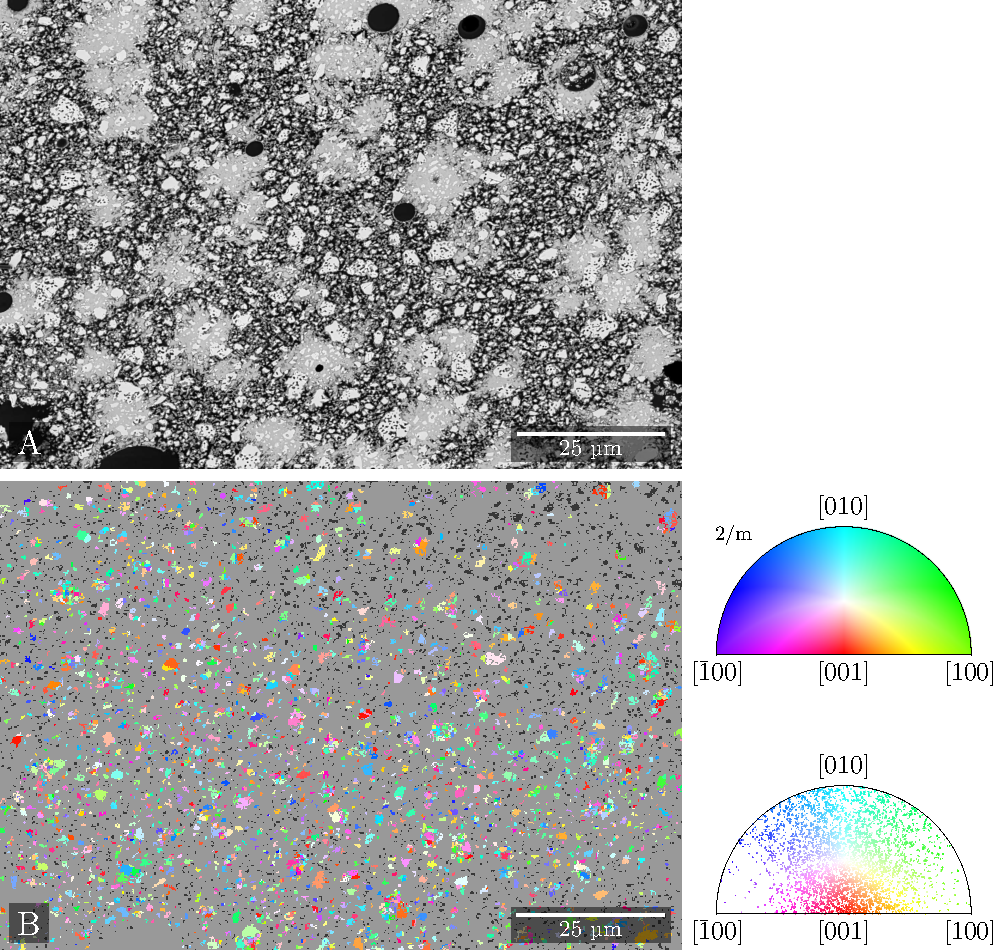
\includegraphics[width=.65\textheight]{./graphics/ebsd/BSE+EBSD-site5.pdf}\\ % fig:ebsd_site5
      \footnotesize BSE- (oben) und EBSD-Mapping (unten)\\mit IPF-Z-Key und IPF-Z-Verteilung
    \end{column}
  \end{columns}
  \vfill\raggedleft\tiny\itshape unpublished
\end{frame}

\begin{frame}{EBSD \& HLT Korrelation}
  \begin{columns}
    \begin{column}{0.4\textwidth}
      \textbf{Ergebnis:}
      \begin{itemize}
        \item Keine starke kristallographische Präferenz gefunden.
        \item Deutliche Messdichtenabhängigkeit von der kristallographischen Orientierung.
        \item Das lokale Umfeld (Porenraum) dominiert das Wachstum.
      \end{itemize}
    \end{column}
    \begin{column}{0.6\textwidth}
      \centering
      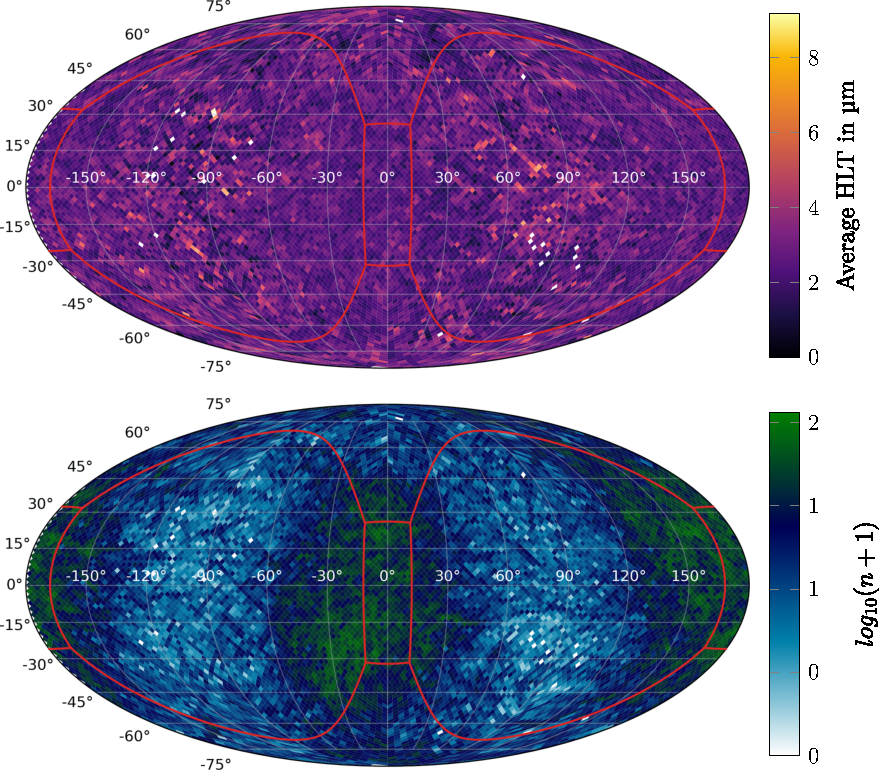
\includegraphics[width=0.7\linewidth]{./graphics/ebsd/mollweideprojektion.pdf}\\ % fig:ebsd_sphere_projection
      \footnotesize Mollweide-Projektion der mittleren HLT (oben) und der Messdichte (unten) mit projizierter \ce{C3S}-Einheitszelle (MIII-Polymorph, rot).
    \end{column}
  \end{columns}
  \vfill\raggedleft\tiny\itshape unpublished
\end{frame}

\subsection{Partikelabstansmessung}
\begin{frame}{Partikelabstände (frischer Leim)}
  \begin{columns}
    \begin{column}{0.5\textwidth}
      \begin{itemize}
        \item Präparation mittels Kryo-FIB-REM zur Erhaltung der nativen Mikrostruktur.
        \item Anpassung des HLT-Algorithmus zur Bestimmung des Partikelabstandes.
      \end{itemize}
      \vspace{0.5cm}
      \textbf{Ergebnisse:}
      \begin{itemize}
        \item Objektive Quantifizierung der Dispergierwirkung.
        \item Effekte von Powerultraschall (PUS) und Fließmitteln (PCE) messbar.
      \end{itemize}
    \end{column}
    \begin{column}{0.5\textwidth}
      \centering
      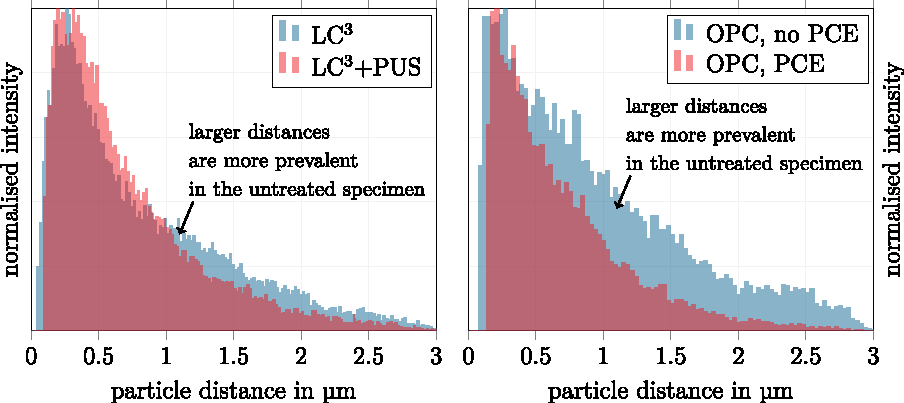
\includegraphics[width=\linewidth]{./graphics/particledistance/diagram.pdf} % fig:cryo-fib-results_2
      \footnotesize Partikelabstandsverteilung von LC$^3$- (links)\\und Portland-Zementpasten (rechts)\\mit und ohne PUS- bzw. PCE-Einsatz.
    \end{column}
  \end{columns}
  \vfill\raggedleft\tiny\itshape unpublished
\end{frame}
    %   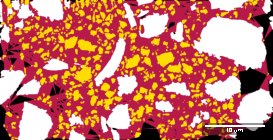
\includegraphics[width=0.48\linewidth]{particle-dist/LC3/noPUS/segmented.pdf}\hfill
    %   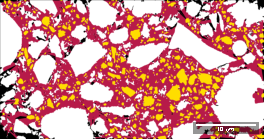
\includegraphics[width=0.48\linewidth]{particle-dist/LC3/PUS/segmented.pdf} % 

    
\section{3D FIB-SEM}    
\subsection{Lift-out Technik}
\begin{frame}{3D Nano-Tomographie (FIB-nT) - Lift-out}
  \begin{columns}
    \begin{column}{0.5\textwidth}
      \textbf{Herausforderungen:}
      \begin{itemize}
        \item Artefakte im Bulk-Material (Charging, Curtaining).
      \end{itemize}
      \textbf{Die Lösung:}
      \begin{itemize}
        \item Lift-out Technik.
        \item Segmentierung mittels 3D SLIC Superpixel \& UMAP Clustering.
        \item MIP/LTDSC-Validierung im Bereich von $\approx$\,10\,nm.
      \end{itemize}
    \end{column}
    \begin{column}{0.5\textwidth}
      \centering
      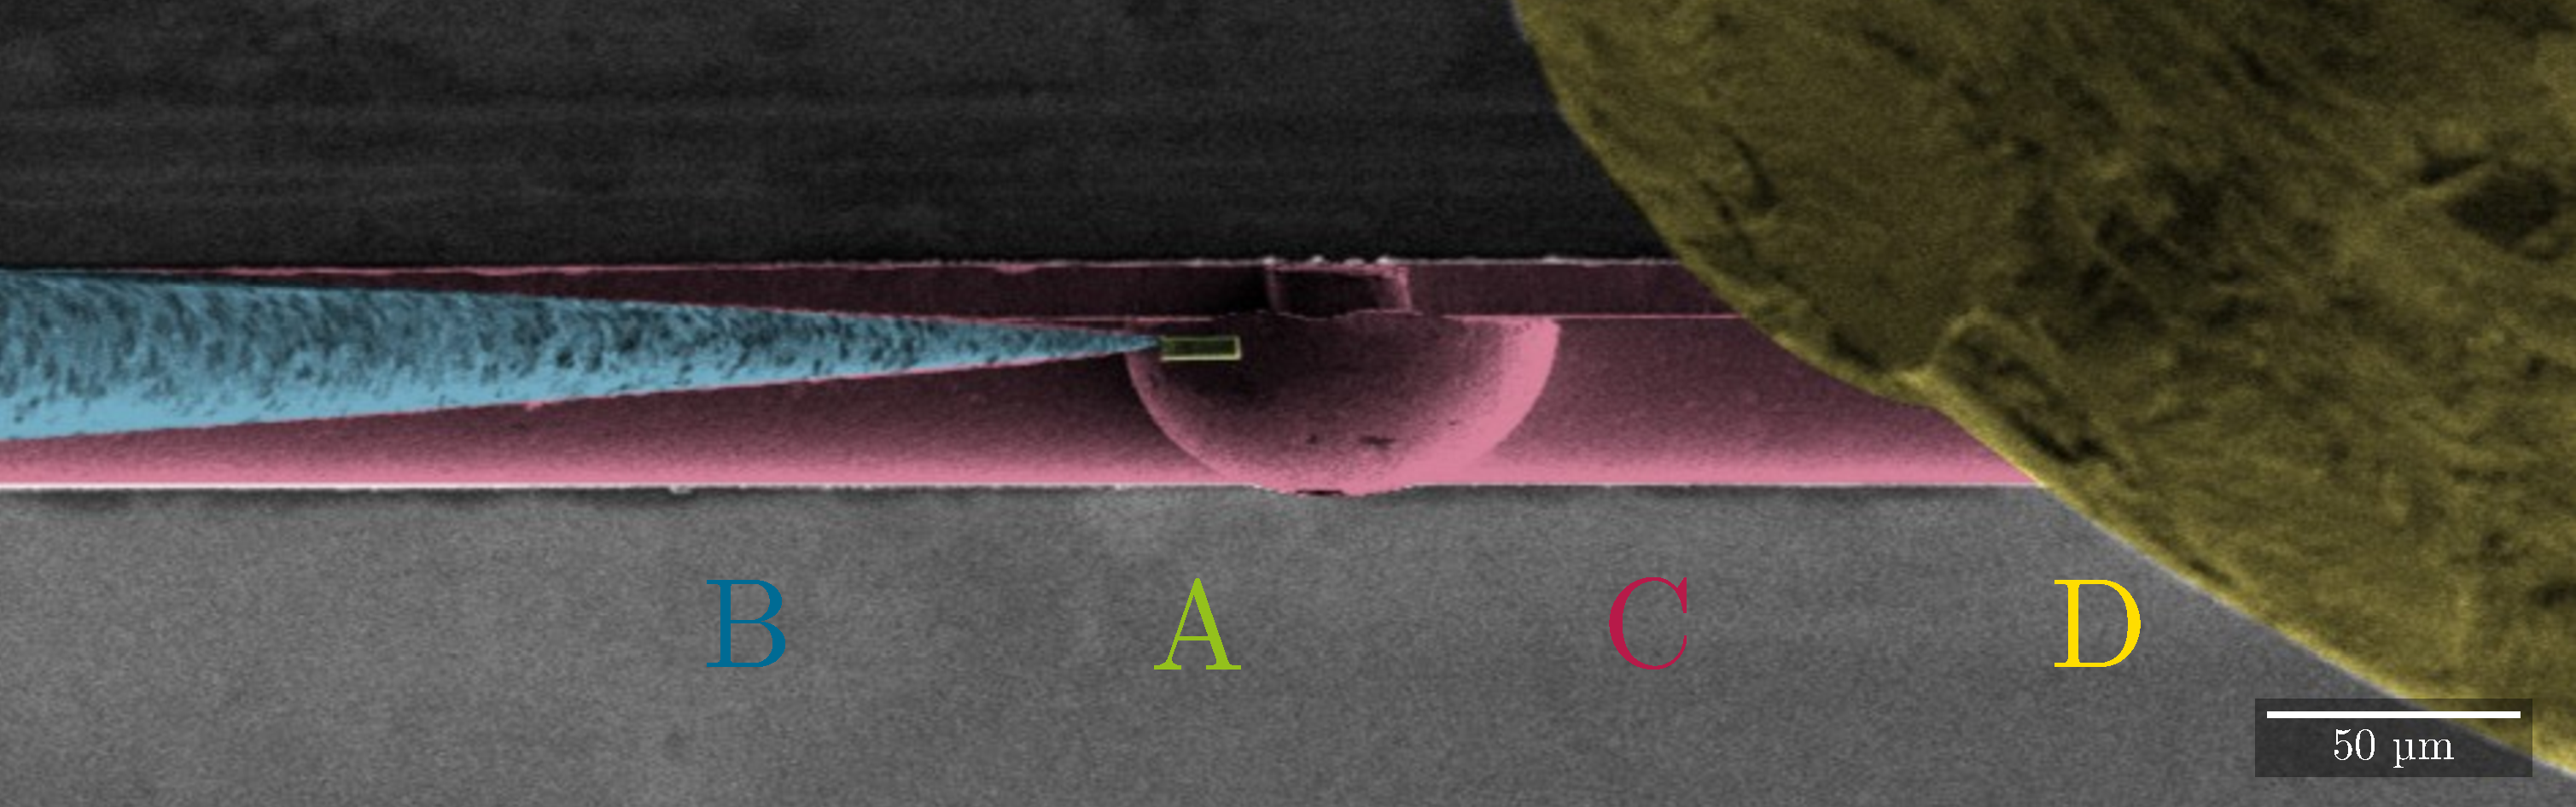
\includegraphics[width=0.9\linewidth]{methods/fib_liftout/image095_colored.pdf} % fig:fig:fib_liftout
      \footnotesize Lift-out Prinzip. A Probe, B Nadel, C Kupferkamm, D Platin-Beschichtungssystem\\[0.2cm]
      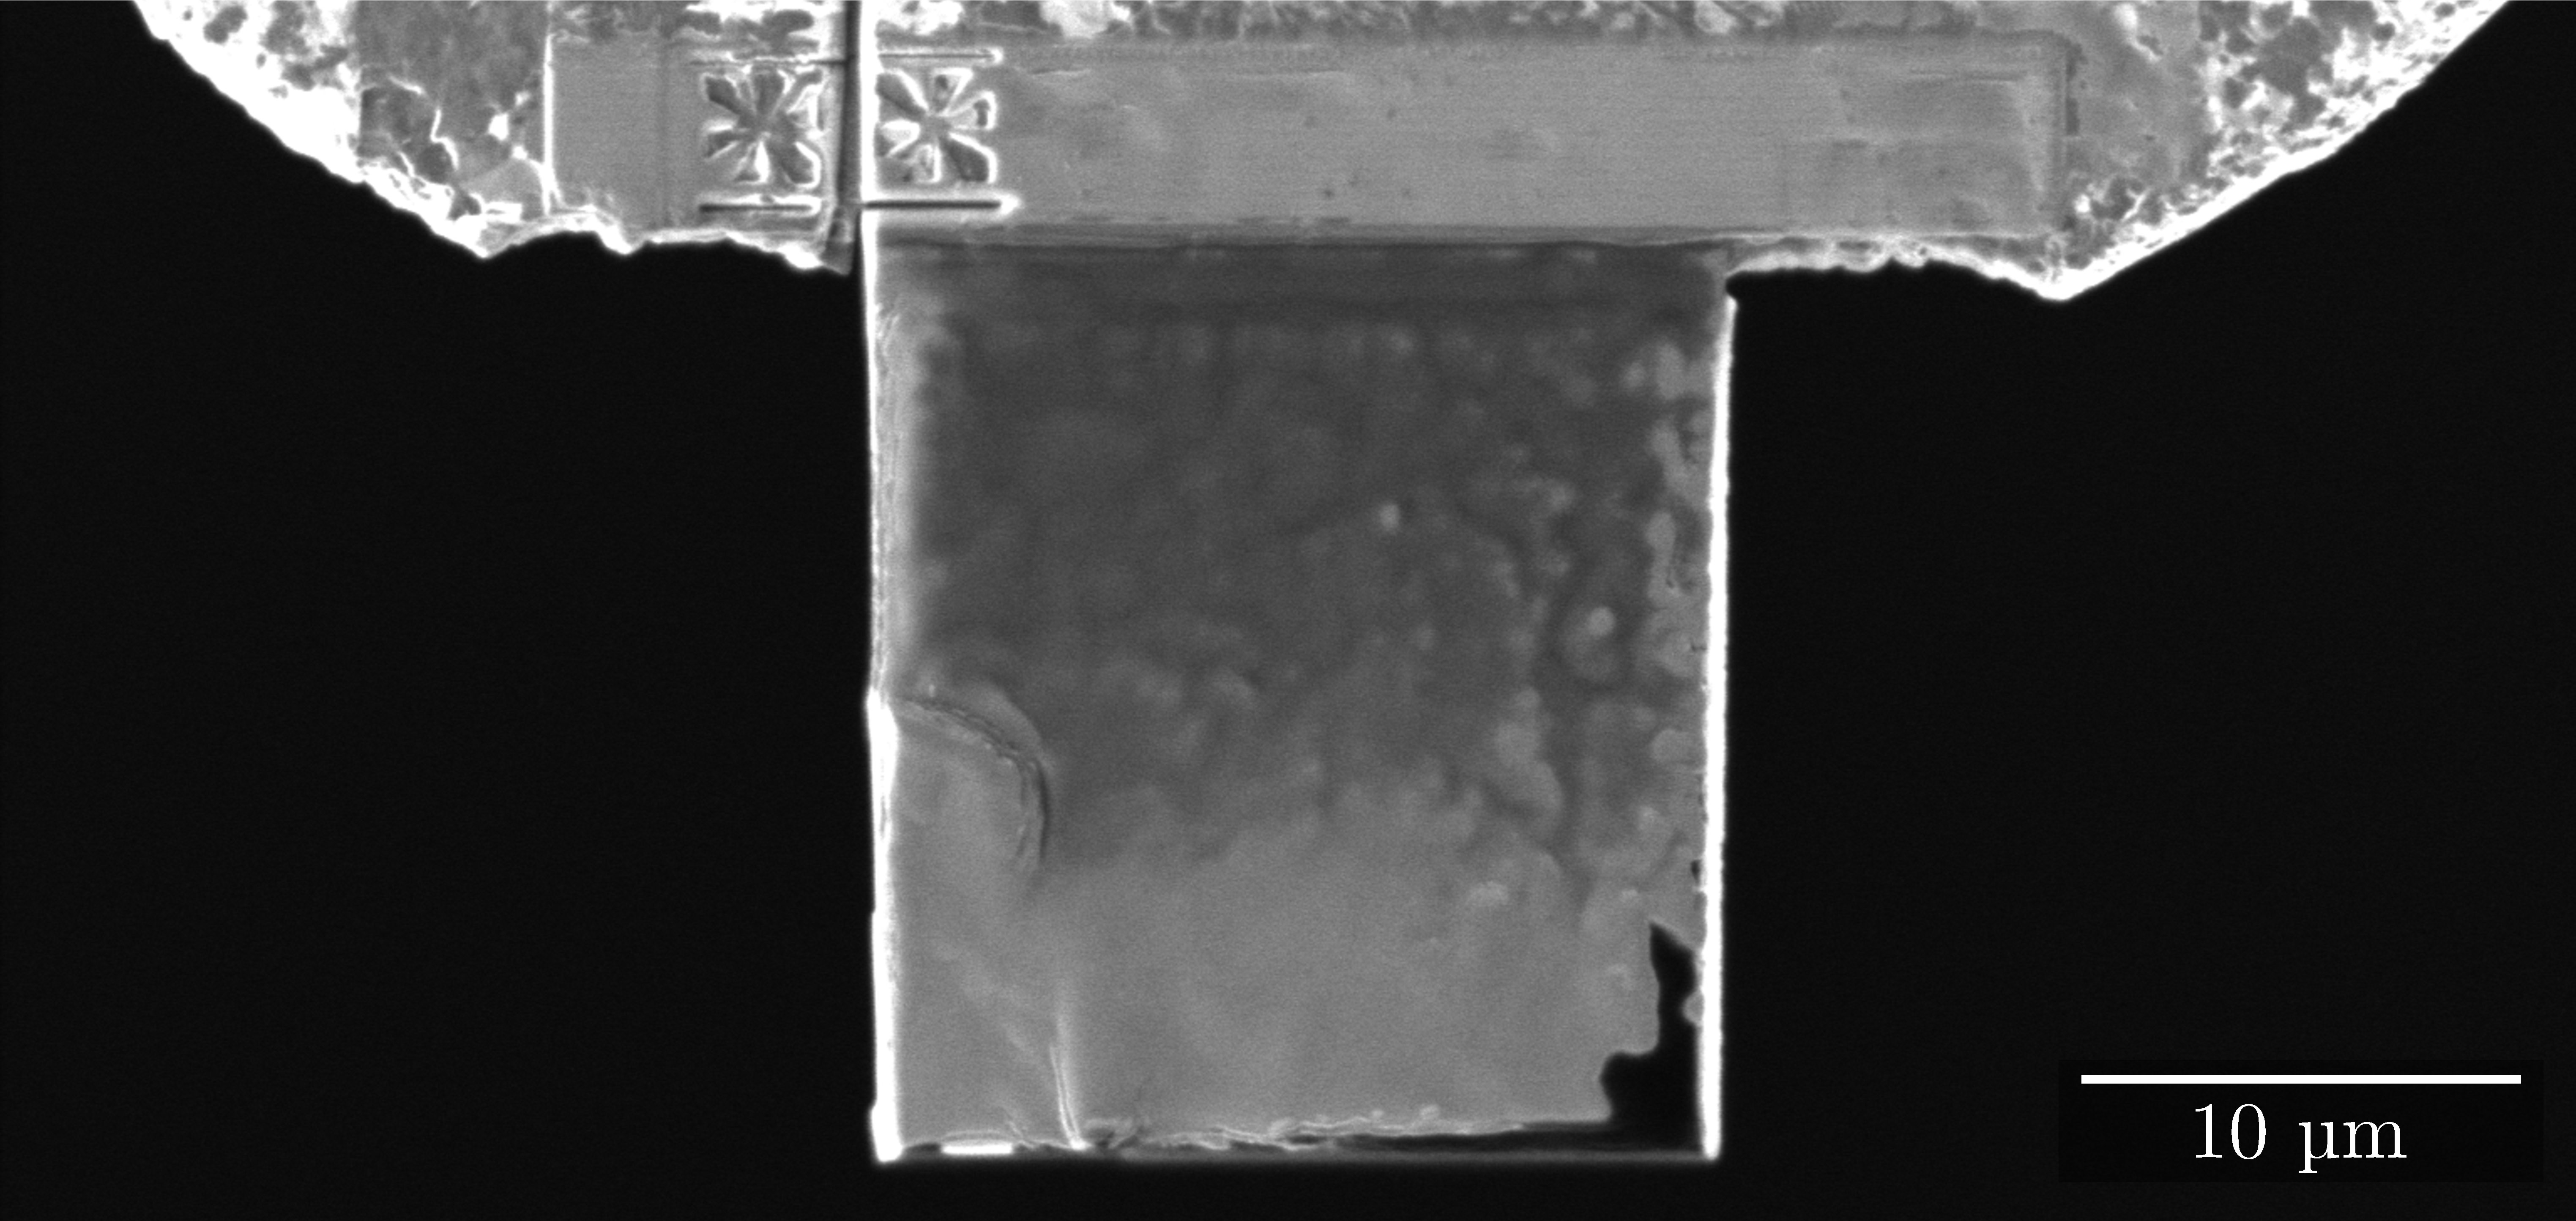
\includegraphics[width=0.65\linewidth]{methods/fib_liftout/ion_image.pdf}\hfill
      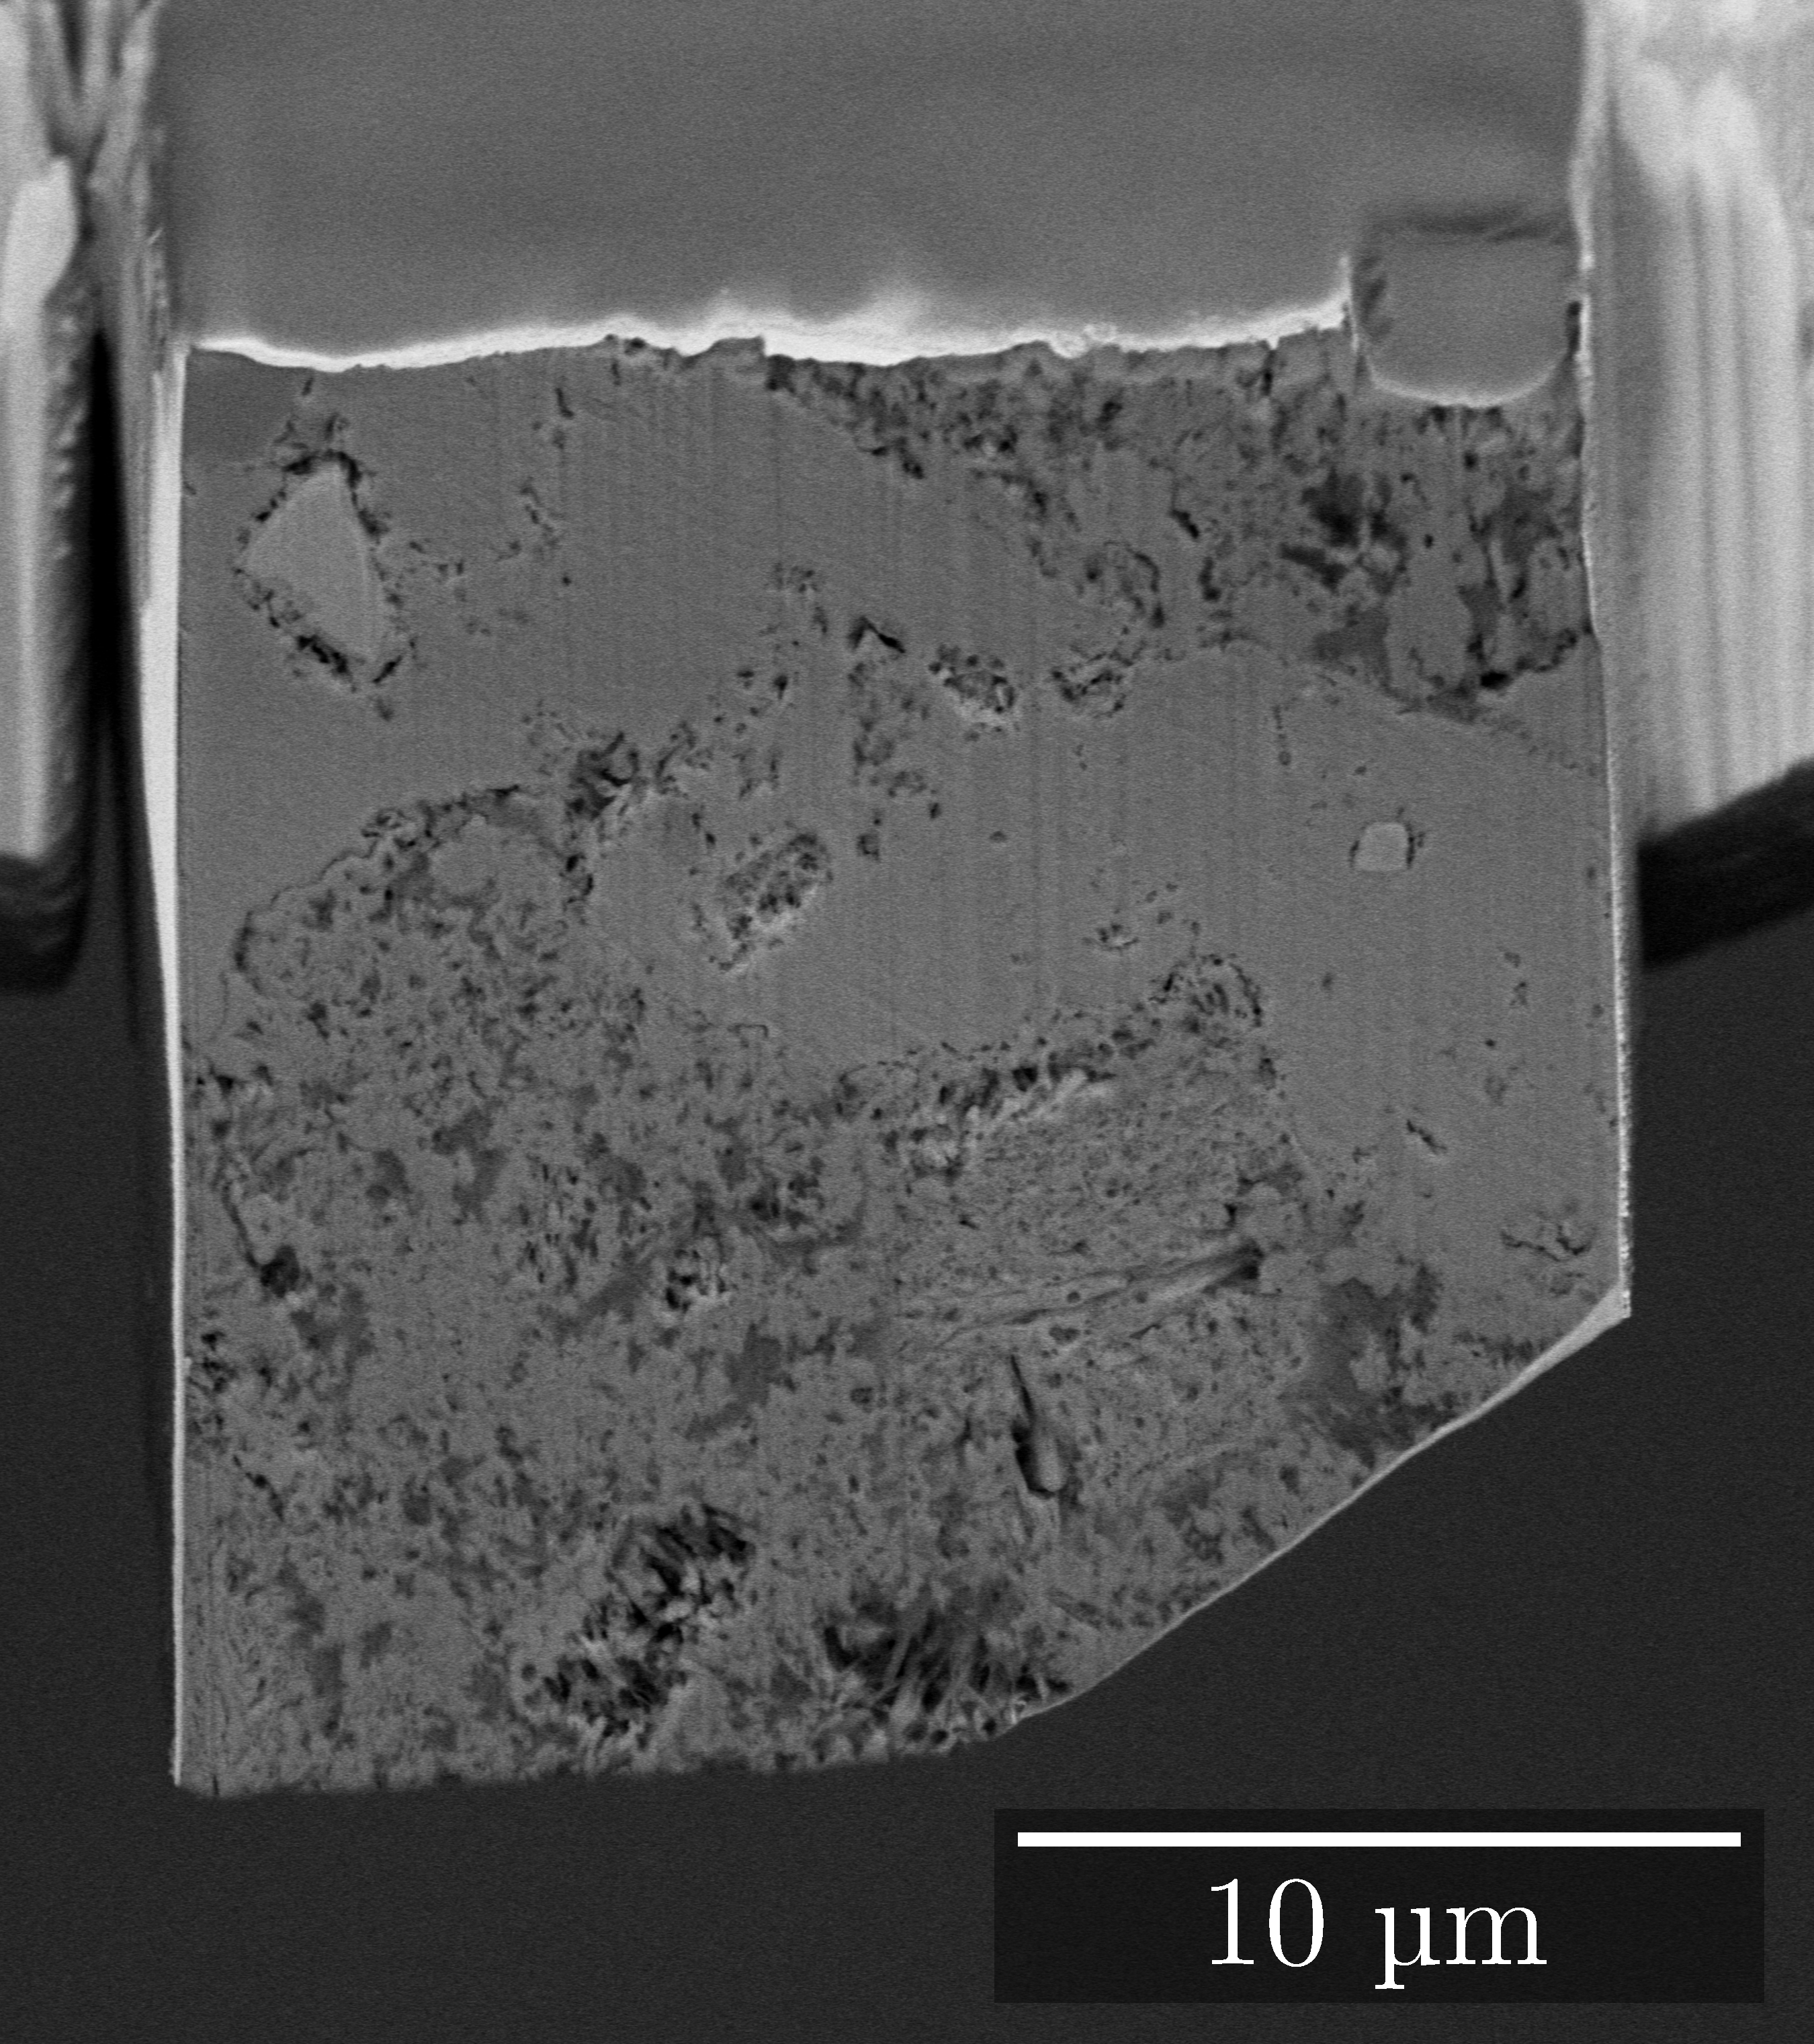
\includegraphics[width=0.27\linewidth]{methods/fib_liftout/bse_image.pdf}\\
      \footnotesize Draufsicht (Ionenbild, links) und\\Frontansicht (BSE, rechts)\\
    \end{column}
  \end{columns}
   \vfill
   \raggedleft\tiny\itshape F. Kleiner, C. Rößler, H.-M. Ludwig,`A FIB-SEM Protocol for High-Resolution Imaging Combined with EDX Analysis of Cement-Based Materials with Minimized Damage', 2025, \doi{10.71758/refodat.52}%kleiner.2025c
\end{frame}

\subsection{fs-Laser Präparation}
\begin{frame}{3D Nano-Tomographie (FIB-nT) - fs-Laser Präparation}
  \begin{columns}
    \begin{column}{0.5\textwidth}
      \textbf{Herausforderungen:}
      \begin{itemize}
        \item Lift-out Technik resultiert in sehr kleinen Volumina\\($20\,\times\,20\,\times\,20\,$µm²).
      \end{itemize}
      \textbf{Die Lösung:}
      \begin{itemize}
        \item Vorpräparation mit fs-Laser erlaubt die Präparation von großen Gräben ($0,6\,\times\,1,0\,$mm²).
      \end{itemize}
    \end{column}
    \begin{column}{0.5\textwidth}
      \centering
      \animategraphics[palindrome,poster=6,autoplay,width=0.49\linewidth]{5}{methods/laser_prep/tilt}{0}{6}\hfill
      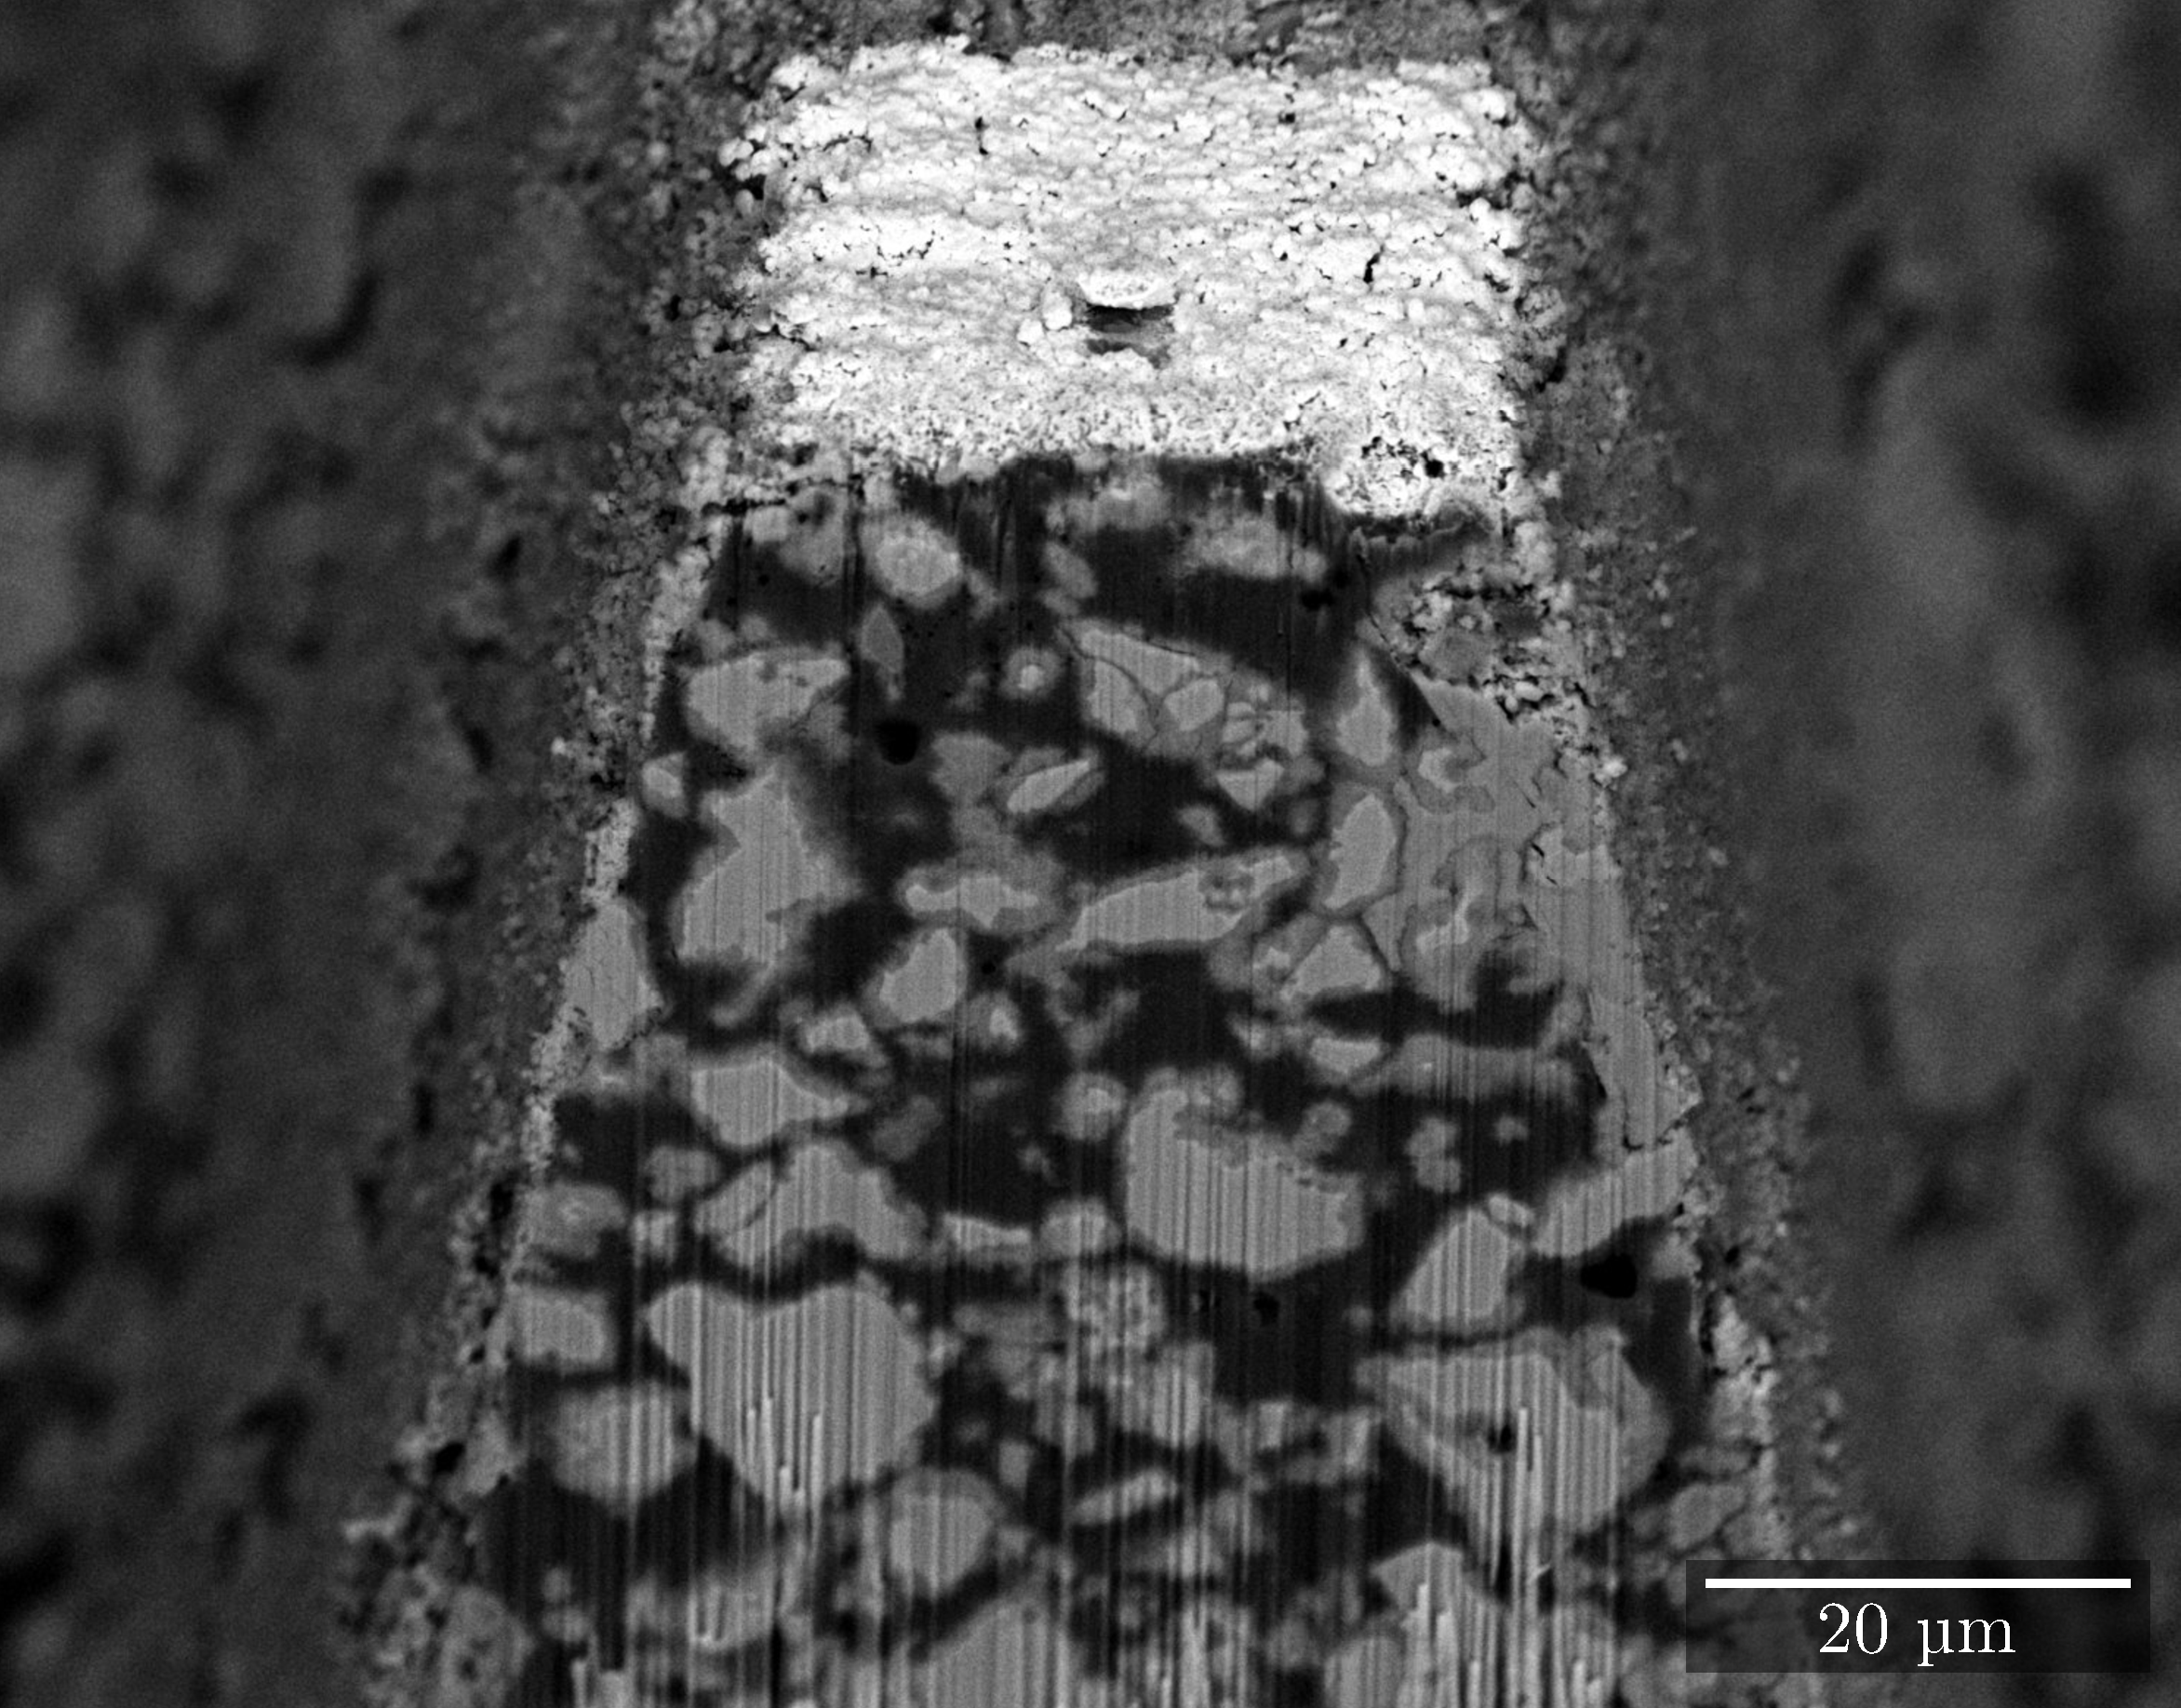
\includegraphics[width=0.49\linewidth]{methods/laser_prep/C3S_7d_Laser_prep_069.pdf}\\
      \footnotesize Laser-Gräben (links) und\\frischer FIB-Schnitt (rechts)\\
    \end{column}
  \end{columns}
  \vfill\raggedleft\tiny\itshape unpublished
\end{frame}

\section{Porenraumanalyse}
\subsection{LTDSC vs. MIP}
\begin{frame}{Porenraumanalyse (LTDSC vs. MIP)}
  \begin{columns}
    \begin{column}{0.5\textwidth}
      \textbf{LT-DSC Auswertung:}
      \begin{itemize}
        \item Bestimmung des Porenvolumens über die Schmelzenthalpie ($\Delta H_{\mathrm{fus}}$).
        \item Differenzierung zwischen Gel- und Kapillarporen ist möglich.
        \item Lineare Abnahme der Kapillarporosität bei gleichzeitiger Zunahme der Gelporosität.
      \end{itemize}
      \textbf{MIP:}
      \begin{itemize}
        \item Primär Kapillarporen ($>10$\,nm)
        \item Porenhals-Effekte
      \end{itemize}
    \end{column}
    \begin{column}{0.5\textwidth}
      \centering
      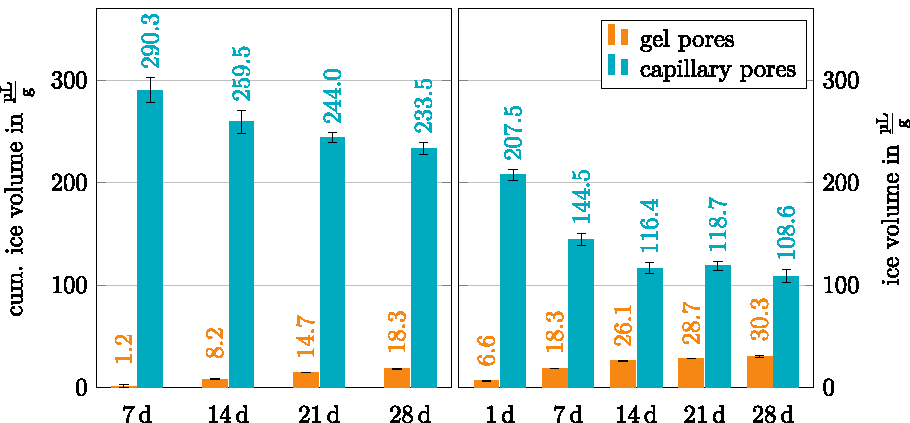
\includegraphics[width=\linewidth]{./graphics/pores/pores.pdf}\\
      \footnotesize Korrelation zwischen Gel- und Kapillarporenvolumen\\bei fortschreitender Hydratation.\\
    \end{column}
  \end{columns}
  \vfill\raggedleft\tiny\itshape unpublished
\end{frame}

\subsection{3D Nano-Porenanalyse (FIB-nT)}
\begin{frame}{3D Nano-Porenanalyse (FIB-nT)}
  \begin{columns}
    \begin{column}{0.5\textwidth}
      \begin{itemize}
        \item Direkte Visualisierung der Porosität innerhalb des dichten C-S-H.
        \item 3D-Rekonstruktion aus hochauflösendem FIB-nT Datensatz.
        \item Dominanter Porenradius bei ca. $10,8$\,nm.
        \item Gute Übereinstimmung mit LT-DSC/MIP und ArBIB-polierten Proben.
      \end{itemize}
    \end{column}
    \begin{column}{0.5\textwidth}
      \centering
      \animategraphics[palindrome,autoplay,width=0.9\linewidth]{10}{fibnt-datasets/vol_ani/volume_}{00}{14}\\
      \footnotesize 3D-Rekonstruktion des Porenraums (grau)\\in C-S-H (rot).
    \end{column}
  \end{columns}
  \vfill\raggedleft\tiny\itshape unpublished
\end{frame}

\section{Zusammenfassung}
\begin{frame}{Zusammenfassung}
  \textbf{Die Arbeit liefert Beispiele für den Einsatz:}
  \begin{itemize}
    \item  von korrelativer Mikroskopie für zementbasierte Materialien.
    \begin{itemize}
        \item Die Kombination (LA-ICP-MS + EDX, HLT + EBSD, NI + EDX) liefert Erkenntnisse, die Einzelmethoden nicht leisten können.
    \end{itemize}
    \item optimierte Präparations- (ArBIB) und 3D-Analyseverfahren (FIB-nT).
    \item automatiserte quantitative Bildanalyseverfahren zur Hydratsaum- und Partikelabstandsmessung.
    \item Porenstrukturanalyse von Nanoporosität mittels FIB-nT und LT-DSC.
  \end{itemize}
\end{frame} 

% ---------------------------------------------------
% BACKUP FOLIEN
% ---------------------------------------------------

\appendix

\begin{frame}{Acronyms}
  \begin{multicols}{2}
    \scriptsize
    \begin{description}[LA-ICP-MS]
      \item[ArBIB] Argon Broad Ion Beam
      \item[BSE] Backscattered Electron
      \item[C-A-S-H] Calcium Aluminate Silicate Hydrate
      \item[CEM~I] Portland cement as defined in DIN EN 197-1
      \item[C-S-H] Calcium Silicate Hydrate
      \item[\ce{C2S}] Dicalcium Silicate
      \item[\ce{C3S}] Tricalcium Silicate
      \item[EBSD] Electron Backscatter Diffraction
      \item[EDX] Energy-Dispersive X-ray Spectroscopy
      \item[FIB] Focussed Ion Beam
      \item[FIB-nT] FIB nano Tomography
      \item[fs-Laser] Femtosecond Laser
      \item[HLT] Hydrate Layer Thickness
      \item[IPF] Inverse Pole Figure
      \item[ITZ] Interfacial Transition Zone
      \item[LA-ICP-MS] Laser Ablation - Inductively Coupled Plasma - Mass Spectrometry
      \item[LC$^3$] Limestone Calcined Clay Cement
      \item[LT-DSC] Low Temperature - Differential Scanning Calorimetry
      \item[MIP] Mercury Intrusion Porosimetry
      \item[NI] Nanoindentation
      \item[PCE] Polycarboxylate Ether
      \item[PUS] Power Ultrasound
      \item[SE] Secondary Electron
      \item[SEM] Scanning Electron Microscope
      \item[SLIC] Simple Linear Iterative Clustering
      \item[UMAP] Uniform Manifold Approximation
    \end{description}
  \end{multicols}
\end{frame}

\end{document}
